\section{Synthetic Task: Further Details}
\label{app:synth}

In this task, we replicate a misspecified synthetic data experiment from \citet{huang2024decisionfocusedPG}. 
Here $X \sim \text{Unif}(0,2)$, and $Y = f^*(X)+ 0.5 - \zeta $, where $\zeta$ is an exponential random variable with mean 0.5. The function $f^*(x)$ denotes the \emph{true} mean of $Y$ as a function of $x$. We set it to a piecewise linear function:
\begin{equation}
    f^*(x) =
\begin{cases}
-4x + 2, & \text{for } x \in [0,\,0.55], \\
-0.2, & \text{for } x \in [0.55,\,2].
\end{cases}
\end{equation}
Sample data are shown in in Figure \ref{fig:synth_data}.
This equation is reflected about the x-axis from provided equations in \citeauthor{huang2024decisionfocusedPG}, but \emph{matches}  their code. % from the supplement. 

The decision task here is to select a binary $z$ value ($\mathcal{Z} = \{ 0, 1\})$ so the cost $c(z, y) {=} z \cdot y$ is minimized. The true data-generating process $f^*(x)$ is only \text{above zero} when $x < 0.5$. Thus, to minimize expected cost, we ideally guess $z=0$ when $x < 0.5$ and $z=1$ otherwise.

\textbf{Model.} We use a 2-parameter linear model: $\hat{y}_{\theta}(x) = \theta_1 x + \theta_0$. While misspecified, by design it can still yield optimal decisions. As long as the learned zero-crossing occurs at $x=0.5$, there are many possible $\theta$ which would achieve optimal cost.

\begin{figure}[!h]
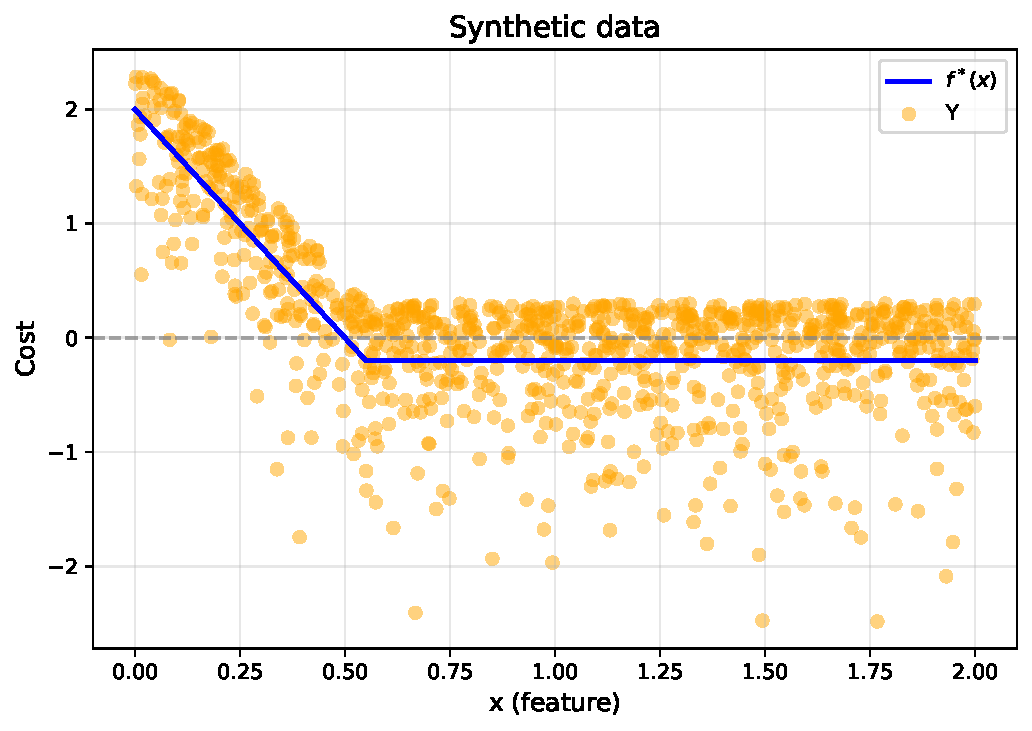
\includegraphics[width=0.65\linewidth]{figures/synthetic_data.pdf}
\caption[Synthetic data task: true mean function $f^*(x)$ and sampled $y$ values with Exponential noise.]{Synthetic data task: True data-generating mean function $f^*(x)$ and sampled $y$ values using zero-mean noise from an Exponential distribution.
In order to minimize cost $z \cdot y$ by taking actions $z \in \{0, 1\}$, the optimal policy is to choose $z{=}0$ when $x<0.5,$ and $z{=}+1$ otherwise. However, the asymmetric noise in $y$ means that, even optimal decisions may sometimes incur a positive cost at any $x$ value; the optimal policy's expected cost is roughly 0.39. }
\label{fig:synth_data}
\end{figure}
